\chapter{Procedura di ottimizzazione}\label{ch:ottimizzazione}
In questo capitolo si descrive la procedura utilizzata e descritta schematicamente nel Capitolo~\ref{ch:math}, per ottimizzare i parametri del modello. Poiché si tratta di un modello non lineare che descrive lo scambio transmembrana di soluti contemporaneamente presenti nello stesso ambiente, non è improbabile che alcuni parametri introdotti specificatamente per un soluto possano influenzare indirettamente anche la dinamica di altri soluti. È quindi necessario stabilire delle \textit{regole} di ottimizzazione, che ci permettano di assegnare un ordine gerarchico ai parametri e di capire in che misura ogni parametro influenza ogni soluto. Si è scelto di ricavare queste regole sfuttando le informazioni derivanti dall'analisi di sensitività del modello.

\section{Analisi di sensitività}\label{sec:sensitivity}
L'analisi di sensitività serve a stabilire quanto i parametri utilizzati in un modello ne influenzino l'uscita. L'argomento è molto vasto e complesso e di non semplice applicazione \cite{bib:sensitivity, hemez, myung}, e in questo sede se ne sfrutteranno le potenzialità, al fine di individuare opportune regole di ottimizzazione dei parametri del modello sviluppato. Non si indagheranno invece né il problema dell'\textit{identificabilità strutturale} dei parametri né l'eventuale loro ridondanza \cite{khoo}.

Limitatamente alle uscite di nostro interesse (le concentrazioni plasmatiche dei soluti) e ai parametri di nostro interesse ($\rho$, $k$, $\eta$) possiamo valutare la variazione di ogni uscita rispetto alla variazione di ogni parametro, costruendo una \textit{matrice di sensitività} \textbf{S} formata dagli elementi:
$$S_{ij}=\frac{\partial y_j}{\partial \theta_i}$$
in cui con $y_j$ si è indicata la cancentrazione plasmatica a fine dialisi del soluto \textit{j}-esimo, e con $\theta_i$ il parametro \textit{i}-esimo. Si precisa che le $N$ uscite da valutare sono le concentrazioni plasmatiche dei $9$ soluti studiati, proteine incluse. I parametri $\theta_i$ sono invece di tre tipi: uno generale ($\rho$) e due specifici ($k$, $\eta$) per ogni soluto, proteine escluse\footnote{per ipotesi la massa (non la concentrazione) delle proteine all'interno di ogni compartimento è ritenuta costante lungo il corso della dialisi, perché si ritiene che siano impermeabili alla membrana cellulare, capillare e a quella del dializzatore. Non ha senso quindi introdurre per le proteine dei parametri che ne descrivono il trasporto attraverso le rispettive membrane.}. In totale vi sono quindi $2(N-1)+1$ parametri da valutare, cioè $17$ parametri. La matrice \textbf{S} è pertanto una matrice con $17$ righe e $9$ colonne.

Poiché si sta trattando un modello numerico, e quindi discreto, bisogna approssimare le derivate necessarie al calcolo degli elementi di \textbf{S} con dei rapporti incrementali. È possibile sfruttare la teoria delle serie di Taylor e approssimare le derivate $\partial y_j/\partial \theta_i$ con una precisione del secondo ordine. Si considerino le relazioni:
\begin{align*}
	&y       = y(\theta,\cdots) \\
	&y^+     = y(\theta + \delta,\cdots) \\
	&y^-     = y(\theta - \delta,\cdots)
\end{align*}
Per ogni coppia \textit{i}, \textit{j} si possono scrivere le seguenti espansioni in serie di Taylor:
\begin{align*}
	&y_j^+         = y_j + \frac{\partial y_j}{\partial \theta_i}\cdot\delta_i + \frac{\partial^2 y_j}{\partial \theta_i^2}\cdot\frac{\delta_i^2}{2} + O(\delta_i^2) \\
	&y_j^-         = y_j - \frac{\partial y_j}{\partial \theta_i}\cdot\delta_i + \frac{\partial^2 y_j}{\partial \theta_i^2}\cdot\frac{\delta_i^2}{2} + O(\delta_i^2) \\
	&y_j^+ - y_j^- = 2\delta_i\cdot\frac{\partial y_j}{\partial \theta_i} + O(\delta_i^2)
\end{align*}
da cui è possibile ricavare un'espressione approssimata al secondo ordine per calcolare gli elementi della matrice \textbf{S}:
\begin{equation}\label{eq:taylor}
	S_{ij} = \frac{\partial y_j}{\partial \theta_i} \approxeq \frac{y_j^+ - y_j^-}{2\delta_i}
\end{equation}
Le derivate dell'equazione precedente devono essere calcolate in un punto di riferimento, identificato dal vettore $\mathbf{\theta_{ref}}$. Gli elementi di $\mathbf{\theta_{ref}}$ sono i $17$ parametri di riferimento, ricavati dalla letteratura o per mezzo di ipotesi; in particolare tutti i parametri $k$, eccetto quello della creatinina, sono stati ricavati da fonti bibliografiche \cite{casagrande, gatti}. Per la creatinina si è ipotizzato un valore di un ordine di grandezza inferiore a quello dell'urea\footnote{il parametro $k$ è il coefficiente di diffusione attraverso la membrana cellulare (\textsection~\ref{trasp_cel}). Si ipotizza che il rapporto di compartimentazione $\beta$ (\textit{ibidem}) sia inversamente proporzionale a $k$ e, poiché $\beta_{creatinina}$ è più grande di circa un ordine di grandezza rispetto a $\beta_{urea}$ (\ref{tab:osmolarit}), si è ipotizzato per $k_{creatinina}$ un valore dieci volte inferiore a $k_{urea}$.}. Il parametro $\rho$ è stato scelto pari a $1$, in quanto tale valore attribuisce alla permeabilità capillare lo stesso valore utilizzato in Ursino et al. \cite{ursino}. I parametri $\eta$ sono stati scelti tutti pari a $0,5$. Gli incrementi $\pm\delta_i$ sono stati presi pari al $\pm 10\%$ dei valori nominali dei parametri $\theta_i$.
\begin{figure}[!b]
	\centering
		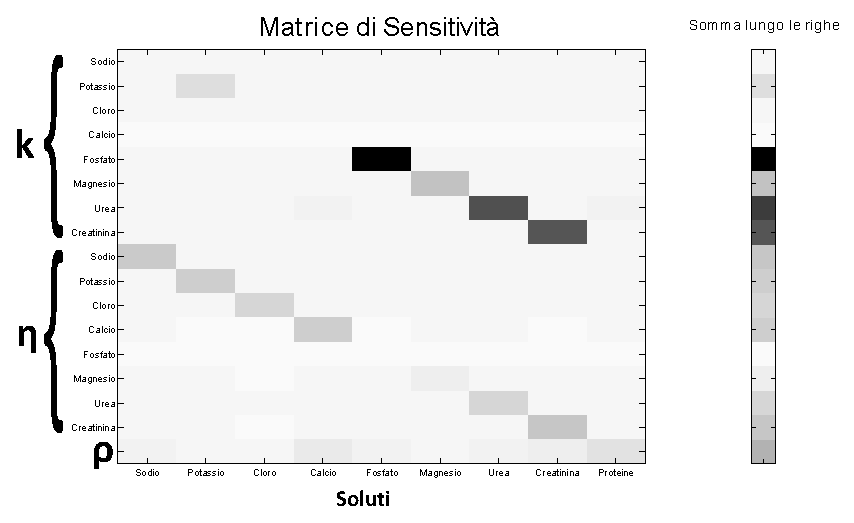
\includegraphics[width=0.9\textwidth]{immagini/sens.eps}
				\caption{Matrice di sensitività di un paziente generico. La somma lungo le righe di \textbf{S} è usata come criterio di ordine per la fase di ottimizzazione. Codice colori: scala di grigio lineare da zero (bianco) al valore massimo (nero).}\label{fig:sens}
\end{figure}

In \figurename~\ref{fig:sens} è mostrato, a titolo esemplificativo, il risultato del calcolo della matrice \textbf{S} per un paziente generico. Per rendere immediatamente interpretabile la matrice, i valori numerici sono stati convertiti in scala di grigio, in cui al bianco corrisponde sensitività nulla e al nero sensitività massima. Dalla figura si nota immediatamente che in questo particolare caso il parametro $k$ del fosfato ha la massima influenza sull'uscita stessa del fosfato, mentre i parametri $k$ del calcio e $\eta$ del fosfato non hanno alcuna influenza su nessuna uscita considerata del modello, pertanto potrebbero anche essere omessi dalla fase di ottimizzazione.

La matrice di sensitività tende a svilupparsi maggiormente lungo le diagonali, indice del fatto che ogni parametro specificatamente introdotto per un particolare soluto ha la sua massima influenza su quel soluto. Al di fuori delle diagonali ci sono comunque livelli di grigio che stanno ad indicare ciò che si è anticipato all'inizio del capitolo, e cioè che esiste una interazione non trascurabile fra i parametri di un particolare soluto e le variazioni di altri soluti.

\section{Ottimizzazione}
La difficoltà dell'ottimizzazione dei parametri $\theta_i$ è imputabile alla loro numerosità: serve un criterio per stabilire in che ordine è più opportuno ottimizzarli. Il procedimento è paragonabile all'operazione di voler pesare una massa sconosciuta utilizzando una bilancia a due bracci servendosi di alcuni pesi campione ($1$ $kg$, $100$ $gr$, $1$ $gr$ \dots). La procedura più rapida è quella di utilizzare per primi i pesi campione più pesanti e successivamente affinare la misura coi pesi campione più leggeri. Allo stesso modo, utilizzando la matrice \textbf{S}, possiamo individuare quali siano i parametri più  influenti e ottimizzarli per primi. La somme dei contributi lungo le righe di \textbf{S} è un indice di questa ``influenza''. Così facendo è possibile ottenere il vettore colonna mostrato a destra della matrice \textbf{S} in \figurename~\ref{fig:sens}. Ordinando il vettore dal parametro più pesante a quello più leggero, ovvero dal colore più scuro a quello più chiaro, si è stabilito un plausibile ordine per ottimizzare in sequenza i parametri $\theta_i$.

Il passo successivo è quello di costruire delle \textit{criterion function} opportune che minimizzate restituiscano come valore il parametro ottimo cercato (\textsection~\ref{sec:simplex}). Si utilizzerà come criterion function \textit{i}-esima la seguente funzione:
\begin{equation}\label{eq:Ji}
	J_i = \sum_{j=1}^N E_{ij} \text{\qquad in cui \qquad}  E_{ij} = \sum_t \bigl(y_{j,sim}(\theta_i,t)-y_{j,true}(t)\bigr)^2
\end{equation}
la quale restituisce un valore reale positivo misura del grado di scarto fra simulazione numerica e realtà clinica. Una funzione del genere non tiene conto della diversa influenza di ogni parametro $\theta_i$ sulle diverse uscite, e non diversifica gli scarti $E_{ij}$ in base alla loro importanza relativa. Per tenere invece conto del fatto che ogni parametro ha un effetto diverso su ogni soluto, si può introdurre un vettore di pesi $w_{ij}$ che assegni ad ogni parametro $\theta_i$ una misura del suo effetto sull'uscita $y_j$. La nuova funzione $J_i$ diventa pertanto:
\begin{equation}
	J_i = \sum_{j=1}^N w_{ij} E_{ij}
\end{equation}
mantenendo per $E_{ij}$ la stessa formulazione usata nell'Eq.~(\ref{eq:Ji}). Resta ora il problema di identificare i pesi $w_{ij}$. Si può ancora una volta sfruttare la matrice di sensitivà \textbf{S} e utilizzare come pesi $w_{ij}$ gli elementi dei vettori riga relativi a ogni parametro $\theta_i$, scalati per la somma degli stessi elementi lungo la riga \textit{i}-esima, cioè:
\begin{equation}
	w_{ij} = \frac{S_{ij}}{\sum_j S_{ij}}
\end{equation}
In questo modo si è creata una \textit{matrice dei pesi} \textbf{W} in cui la somma degli elementi lungo le righe dà come risultato $1$, confermando che si tratta di coefficienti di peso ben definiti.
\begin{figure}[!t]
	\centering
		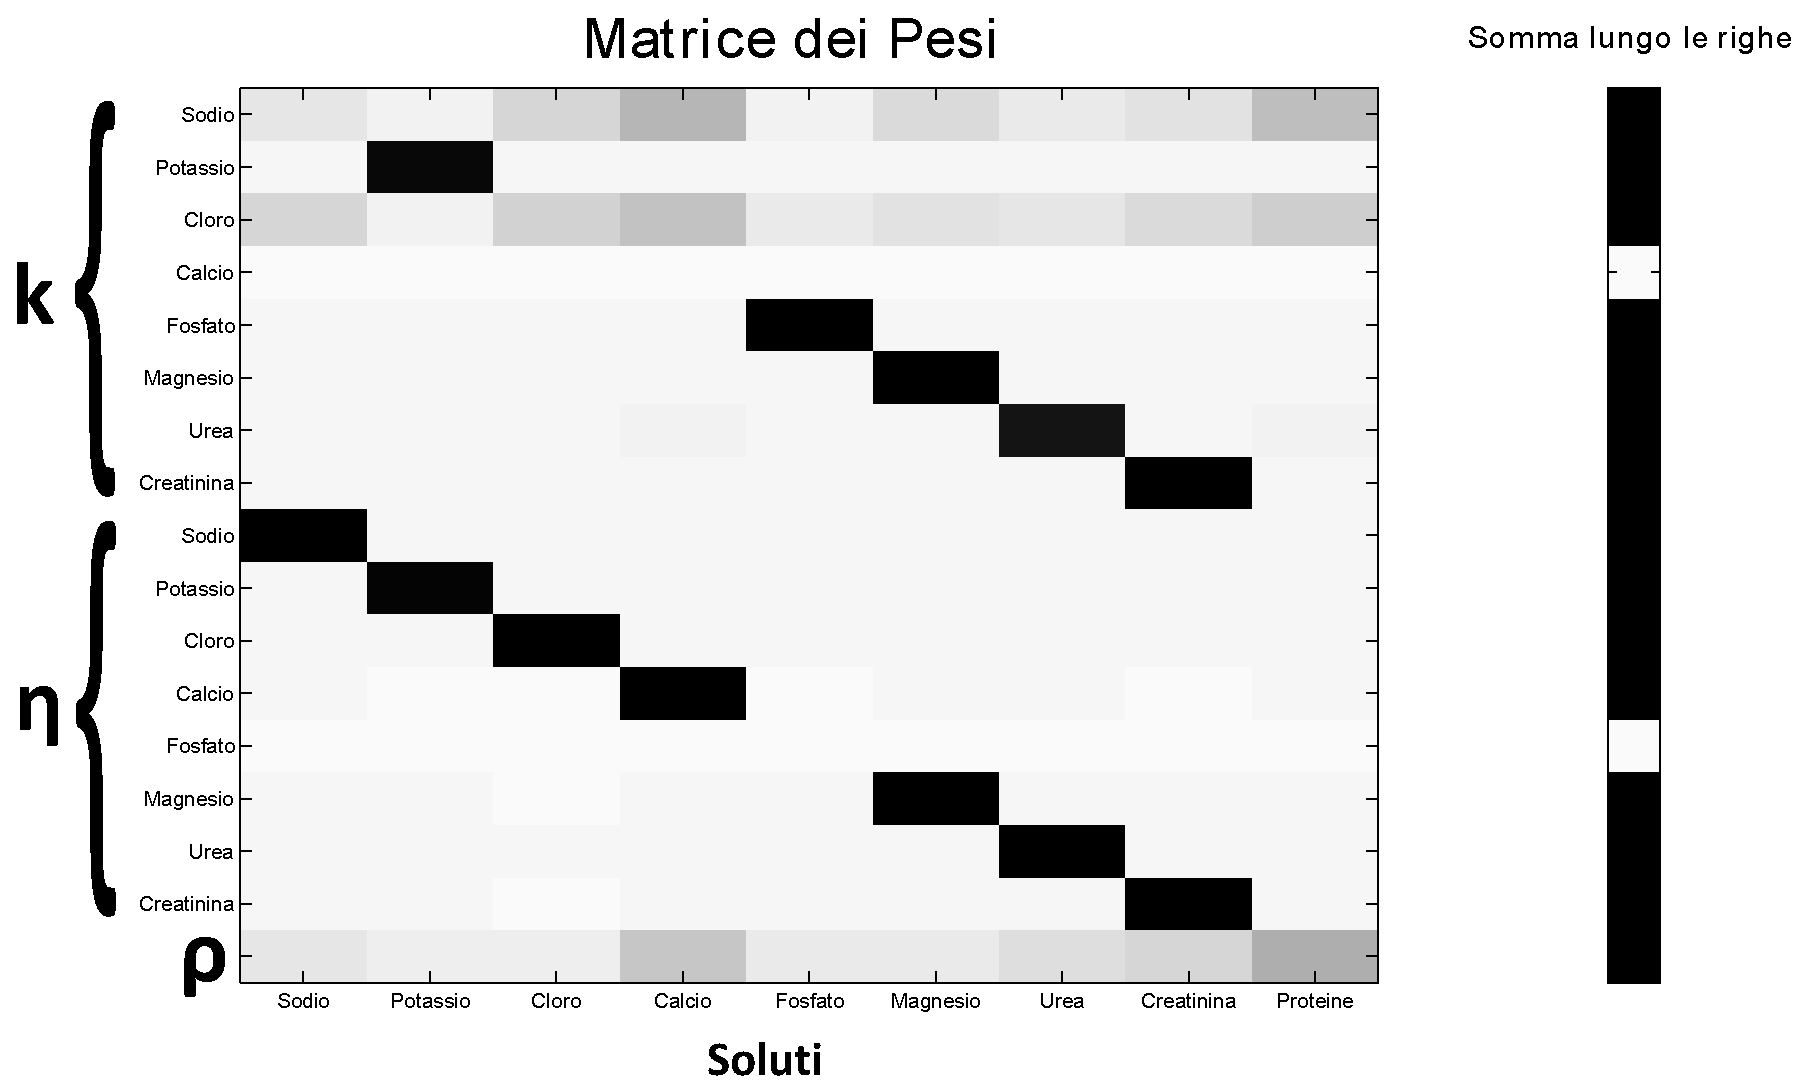
\includegraphics[width=0.9\textwidth]{immagini/pesi.eps}
				\caption{Matrice \textbf{W} dei pesi ricavata dalla matrice \textbf{S}. Scala lineare di grigio: Nero = 1, Bianco = 0. La somma pari a $1$ lungo le righe di \textbf{W} mostra che i pesi dei parametri utili all'ottimizzazione sono ben definiti. I parametri dei pesi a somma nulla sono ininfluenti e pertanto esclusi dall'ottimizzazione.}\label{fig:pesi}
\end{figure}
In \figurename~\ref{fig:pesi} è illustrata la matrice dei pesi ricavata da quella di sensitività. Per la matrice dei pesi il codice dei colori è sempre in scala di grigio lineare dove al nero corrisponde il valore numerico $1$ e al bianco il valore numerico $0$. Si nota che i parametri ininfluenti (in questo particolare caso $k$ del calcio e $\eta$ del fosfato) hanno somma dei pesi pari a zero, e pertanto sono esclusi dalla fase di ottimizzazione.

La matrice \textbf{W} ha un contenuto informativo minore della matrice \textbf{S}, ma mette in risalto delle proprietà dei parametri altrimenti poco visibili. La tendenza alla diagonalizzazione è molto più marcata nella matrice dei pesi, e risultano più evidenti i fenomeni di interazione fra i parametri e i soluti del modello: il parametro $k$ di sodio e cloro e il parametro $\rho$ sembrano avere un'influenza generalizzata e non specifica per un soluto in particolare. Che il parametro $\rho$ mostri questa proprietà è facilmente spiegabile se si considera che si tratta di un parametro generale, che influenza la permeabilità all'acqua della membrana capillare e quindi influenza potenzialmente la concentrazione plasmatica di ogni soluto. Influenza specialmente le proteine la cui massa compartimentata, ritenuta costante, le rende più suscettibili alle variazioni di concentrazione a seguito di trasferimenti di volume fra plasma e interstizio. L'influenza generalizzata sul modello che invece mostrano i parametri di sodio e cloro può essere dovuta al fatto che questi soluti sono quelli che, rispetto a tutti gli altri, hanno una concentrazione plasmatica maggiore (\tablename~\ref{tab:osmolarit}) e quindi sono i soluti che danno il maggior contributo all'osmolarità plasmatica, la quale poi influenza i fenomeni di trasporto che riguardano tutti gli altri soluti.